\documentclass[11pt]{article}
\usepackage[utf8]{inputenc}
\usepackage[margin=1in]{geometry}
\usepackage{mathptmx} % Professional Times New Roman font
\usepackage{amsmath}
\usepackage{amssymb}
\usepackage{amsthm}
\usepackage{enumitem}
\usepackage{graphicx}
\usepackage{booktabs}
\usepackage{algorithm}
\usepackage{algorithmic}

\title{\textbf{Project Report: Convex Relaxation for E-VRPTW}}
\author{Weiqi Zhou, Junhan Chen, Xinzi Huang, Yiqian Liu}
\date{March 2026}

\begin{document}
\maketitle

\section{Introduction}
\textbf{Motivation:} Electric Vehicle (EV) logistics face significant constraints due to limited battery capacity and lengthy recharging times. While heuristic and metaheuristic methods construct feasible routes quickly, they treat the objective as a black box and offer no guarantees of global optimality or theoretical lower bounds to assess solution quality. \\
\textbf{Previous Works:} The foundation of the Electric Vehicle Routing Problem with Time Windows (E-VRPTW) was formally established by Schneider et al. [1], who modeled the core constraints of limited battery capacities and restricted recharging stations, solving it via a hybrid Variable Neighborhood Search (VNS) and Tabu Search heuristic. Building upon this, subsequent research expanded the logistical scope to improve computational and operational efficiency. Verma [2] introduced multi-modal replenishment by integrating battery swapping stations to bypass long recharging times, while Xiao et al. [3] formulated a comprehensive model reflecting nonlinear energy consumption realities.\\

Despite structural advancements, the predominant solution paradigms have remained overwhelmingly heuristic. As highlighted in a recent survey by Zhou et al. [4], the literature heavily favors metaheuristic algorithms designed for rapid, feasible approximations over exact mathematical certifications. A contemporary example is the work of Donval et al. [5], who utilized Ant Colony Optimization with dynamic pheromones to jointly navigate routing and charging decisions. While these heuristic methodologies construct feasible routes effectively, they fundamentally treat the optimization objective as a black box. Very few works rigorously explore the problem's convex geometric properties or apply relaxation techniques to establish definitive theoretical lower bounds, making it difficult to assess absolute solution quality.\\
\textbf{Intended Contributions:} This project pivots from heuristic search to \textbf{Convex Optimization}. By formulating the E-VRPTW as a Mixed-Integer Convex Program (MICP), we apply \textbf{Lagrangian Relaxation} to decouple complex constraints (time windows, load, and battery capacity). This theoretically rigorous approach allows us to establish baseline optimality certificates computationally using Subgradient Optimization.\\
\textbf{Organization:} This report formally defines the Primal integer problem, derives its Dual formulation via Lagrangian Relaxation, and discusses the continuous KKT optimality conditions (Section 2). We then outline our dataset, algorithmic approach, and Subgradient Optimization algorithm (Section 3), concluding with empirical results and duality gap analysis computed across various benchmark instances (Section 4).

\section{Statement of the Problem}
We define the problem on a directed graph $G=(V, A)$. Let $C$ be the customer set, $F$ the charging stations, and node $0$ the depot. The objective is to minimize total travel time/distance for a fleet of $m$ vehicles. Let $x_{ij} \in \{0, 1\}$ equal $1$ if a vehicle travels from node $i$ to $j$. Variables $\tau_i, u_i, y_i$ capture the arrival time, remaining load, and remaining battery upon departure from node $i$. Variables $d_{ij}, t_{ij}, e_{ij}, q_i$ encode distance, travel time, energy cost, and demand respectively.

\subsection{Primal Formulation (Integer/Non-Convex)}
\textbf{Objective:} Minimize the total traveled distance.
\begin{align}
    \min_{x, \tau, u, y} \quad & \sum_{(i,j) \in A} d_{ij} x_{ij} 
\end{align}
\textbf{Subject to:} 
\begin{align}
    \sum_{j \in V} x_{ij} &= 1 & \forall i \in C \label{c:degree}\\
    \sum_{i \in V} x_{ij} - \sum_{i \in V} x_{ji} &= 0 & \forall j \in (C \cup F) \label{c:flow} \\
    \tau_j &\ge \tau_i + s_i + t_{ij} - M_T(1 - x_{ij}) & \forall (i,j) \in A \label{c:time} \\
    u_j &\le u_i - q_i + M_L(1 - x_{ij}) & \forall (i,j) \in A \label{c:load} \\
    y_j &\le y_i - e_{ij} + M_B(1 - x_{ij}) & \forall (i,j) \in A, \, j \notin F \label{c:battery} \\
    RD_i &\le \tau_i \le DD_i & \forall i \in V \\
    0 &\le u_i \le C, \quad 0 \le y_i \le Q & \forall i \in V \\
    x_{ij} &\in \{0, 1\} & \forall (i,j) \in A
\end{align}

\subsection{Dual Formulation (Lagrangian Relaxation)}
To simplify the primal computational burden, we relax the challenging ``Big-M'' coupling constraints (\ref{c:time}), (\ref{c:load}), and (\ref{c:battery}) by bringing them into the objective function. By introducing non-negative Lagrange multipliers $\lambda^T_{ij}, \lambda^L_{ij}, \lambda^B_{ij} \ge 0$, we penalize any violation of the time windows, vehicle load limits, and battery capacities. Note that for the continuous LP relaxation baseline, the binary variables $x_{ij}$ are relaxed to $[0,1]$.

The Lagrangian function is formulated by adding the penalized terms to the original objective:
\begin{footnotesize}
\begin{align*}
    L(x, \tau, u, y, \lambda) = \sum_{(i,j) \in A} d_{ij} x_{ij} 
    &+ \sum_{(i,j) \in A} \lambda^T_{ij} \Big(\tau_i - \tau_j + s_i + t_{ij} - M_T(1 - x_{ij})\Big) \\
    &+ \sum_{(i,j) \in A} \lambda^L_{ij} \Big(u_i - u_j + q_i - M_L(1 - x_{ij})\Big) \\
    &+ \sum_{\substack{(i,j) \in A \\ j \notin F}} \lambda^B_{ij} \Big(y_i - y_j + e_{ij} - M_B(1 - x_{ij})\Big)
\end{align*}
\end{footnotesize}

By rearranging the terms with respect to the continuous variables $\tau, u$, and $y$, the Lagrangian function effectively decouples the structural routing decisions (which nodes to visit) from the temporal and resource-based sequencing decisions.

The \textbf{Lagrangian Dual Function} $g(\lambda)$ is defined by minimizing this Lagrangian over the remaining feasible region $X$:
\[ g(\lambda) = \min_{x, \tau, u, y \in X} L(x, \tau, u, y, \lambda) \]
where $X$ captures the remaining hard constraints: the degree constraints (\ref{c:degree}), flow conservation (\ref{c:flow}), and variable bounding constraints. Because the complicating path-dependent constraints have been relaxed, solving for $g(\lambda)$ simplifies into a Minimum Cost Network Flow Optimization or an Assignment-like structure, which can be solved efficiently.

The \textbf{Lagrangian Dual Problem} aims to find the tightest possible lower bound by maximizing the dual function over all non-negative multiplier combinations:
\begin{align}
    \max_{\lambda \ge 0} \quad g(\lambda)
\end{align}
Because $g(\lambda)$ is the pointwise minimum of a family of affine functions (one for each feasible primal solution), the dual function is piecewise linear and strictly concave. This mathematical property guarantees that we can search for the maximal bound without getting trapped in local maxima, motivating our use of subgradient search techniques.

\subsection{KKT Conditions}
For the continuous LP relaxation ($0 \le x_{ij} \le 1$), the problem satisfies Slater's condition and is strictly convex. A primal-dual pair $(x^*, \tau^*, u^*, y^*, \lambda^*)$ optimally solves the relaxation if and only if it satisfies the Karush-Kuhn-Tucker (KKT) conditions:
\begin{itemize}
    \item \textbf{Primal Feasibility:} Constraints (\ref{c:degree}) -- (\ref{c:battery}) hold with $x_{ij}^* \in [0,1]$.
    \item \textbf{Dual Feasibility:} $\lambda^{T*}_{ij} \ge 0, \lambda^{L*}_{ij} \ge 0, \lambda^{B*}_{ij} \ge 0$.
    \item \textbf{Complementary Slackness:} Multipliers are nonzero only when the primal constraints are tight. E.g., $\lambda^{T*}_{ij} \cdot (\tau_i^* - \tau_j^* + s_i + t_{ij} - M_T(1 - x_{ij}^*)) = 0$.
    \item \textbf{Stationarity:} The gradient of $L(x, \tau, u, y, \lambda^*)$ with respect to the primal continuous variables evaluates to zero (identifying extreme points of the gradient).
\end{itemize}

\section{Intended Approaches}

\subsection{Sample Dataset}
Our analysis utilizes the well-regarded Schneider (2014) \texttt{evrptw\_instances} dataset, specifically focusing on the 5-node and 10-node localized clusters. For each location (depot, recharging station, or customer), the dataset provides:
\begin{itemize}
    \item \textbf{Coordinates \& Distance}: $(x, y)$ coordinates to compute Euclidean inter-location travel times.
    \item \textbf{Demands \& Time Windows}: Freighter capacity requirements ($q_i$) and active operational operational windows ($[RD_i, DD_i]$).
    \item \textbf{EV Logistics Parameters}: Vehicle specific constraints including Load Capacity ($C=200$), Battery Capacity ($Q=77.75$), fuel consumption rate ($r=1.0$), and inverse refueling rate ($g=3.47$).
\end{itemize}

\subsection{Solver Approach}
With non-continuous decisions tracking individual paths across time, our primal formulation is a Mixed-Integer Convex Program (MICP). Standard MILP solvers face severe computational challenges scaling up due to the "Big-M" constraints. By migrating these into the objective through our Lagrangian penalty framework, we efficiently simplify the subproblem. This decoupled subproblem acts strictly as a minimum cost network flow algorithm which can be resolved in polynomial bounds using the \texttt{PuLP} framework atop the CBC solver.

\subsection{Algorithm Logic}
Because the dual function $g(\lambda)$ is piecewise linear and concave, but non-differentiable at junction solutions, standard gradient ascent cannot reliably converge. Thus, we implemented the \textbf{Subgradient Optimization Method}.
\begin{algorithm}[H]
\caption{Subgradient Optimization iteratively solving $g(\lambda)$}
\begin{algorithmic}[1]
\STATE Initialize multipliers $\lambda^T_{ij} = \lambda^L_{ij} = \lambda^B_{ij} = 0$, iteration $k=0$, $\alpha = 2.0$.
\WHILE{$k < K_{max}$ and $\alpha > \epsilon$}
    \STATE Solve Lagrangian Subproblem $g(\lambda^k)$ using CBC LP Solver to obtain primal vector $(x^k, \tau^k, u^k, y^k)$.
    \STATE Evaluate subgradients $v^T, v^L, v^B$ representing constraint violations (e.g. $v^T_{ij} = \tau_i^k - \tau_j^k + \dots$).
    \STATE Calculate step size $\theta^k = \alpha \frac{UB - g(\lambda^k)}{||v^T||^2 + ||v^L||^2 + ||v^B||^2}$.
    \STATE Update multipliers: $\lambda_{ij}^{k+1} = \max(0, \lambda_{ij}^k + \theta^k v_{ij}^k)$.
    \STATE Adjust $\alpha = \alpha / 2$ if no bound improvement occurs over $P$ iterations.
\ENDWHILE
\end{algorithmic}
\end{algorithm}

\section{Results \& Conclusion}
\subsection{Conjectured Results (Duality Gap Analysis)}
We computationally implemented the framework natively using Python's \texttt{PuLP} framework running over the CBC solver engine. We benchmarked the E-VRPTW baseline LP Bound against our proposed subgradient LR Bound upon Schneider et al.'s 2014 synthetic benchmark clusters, specifically targeting exactly valid instances across multiple \texttt{c, r,} and \texttt{rc} clusters with 5 and 10 nodes.

\begin{figure}[H]
    \centering
    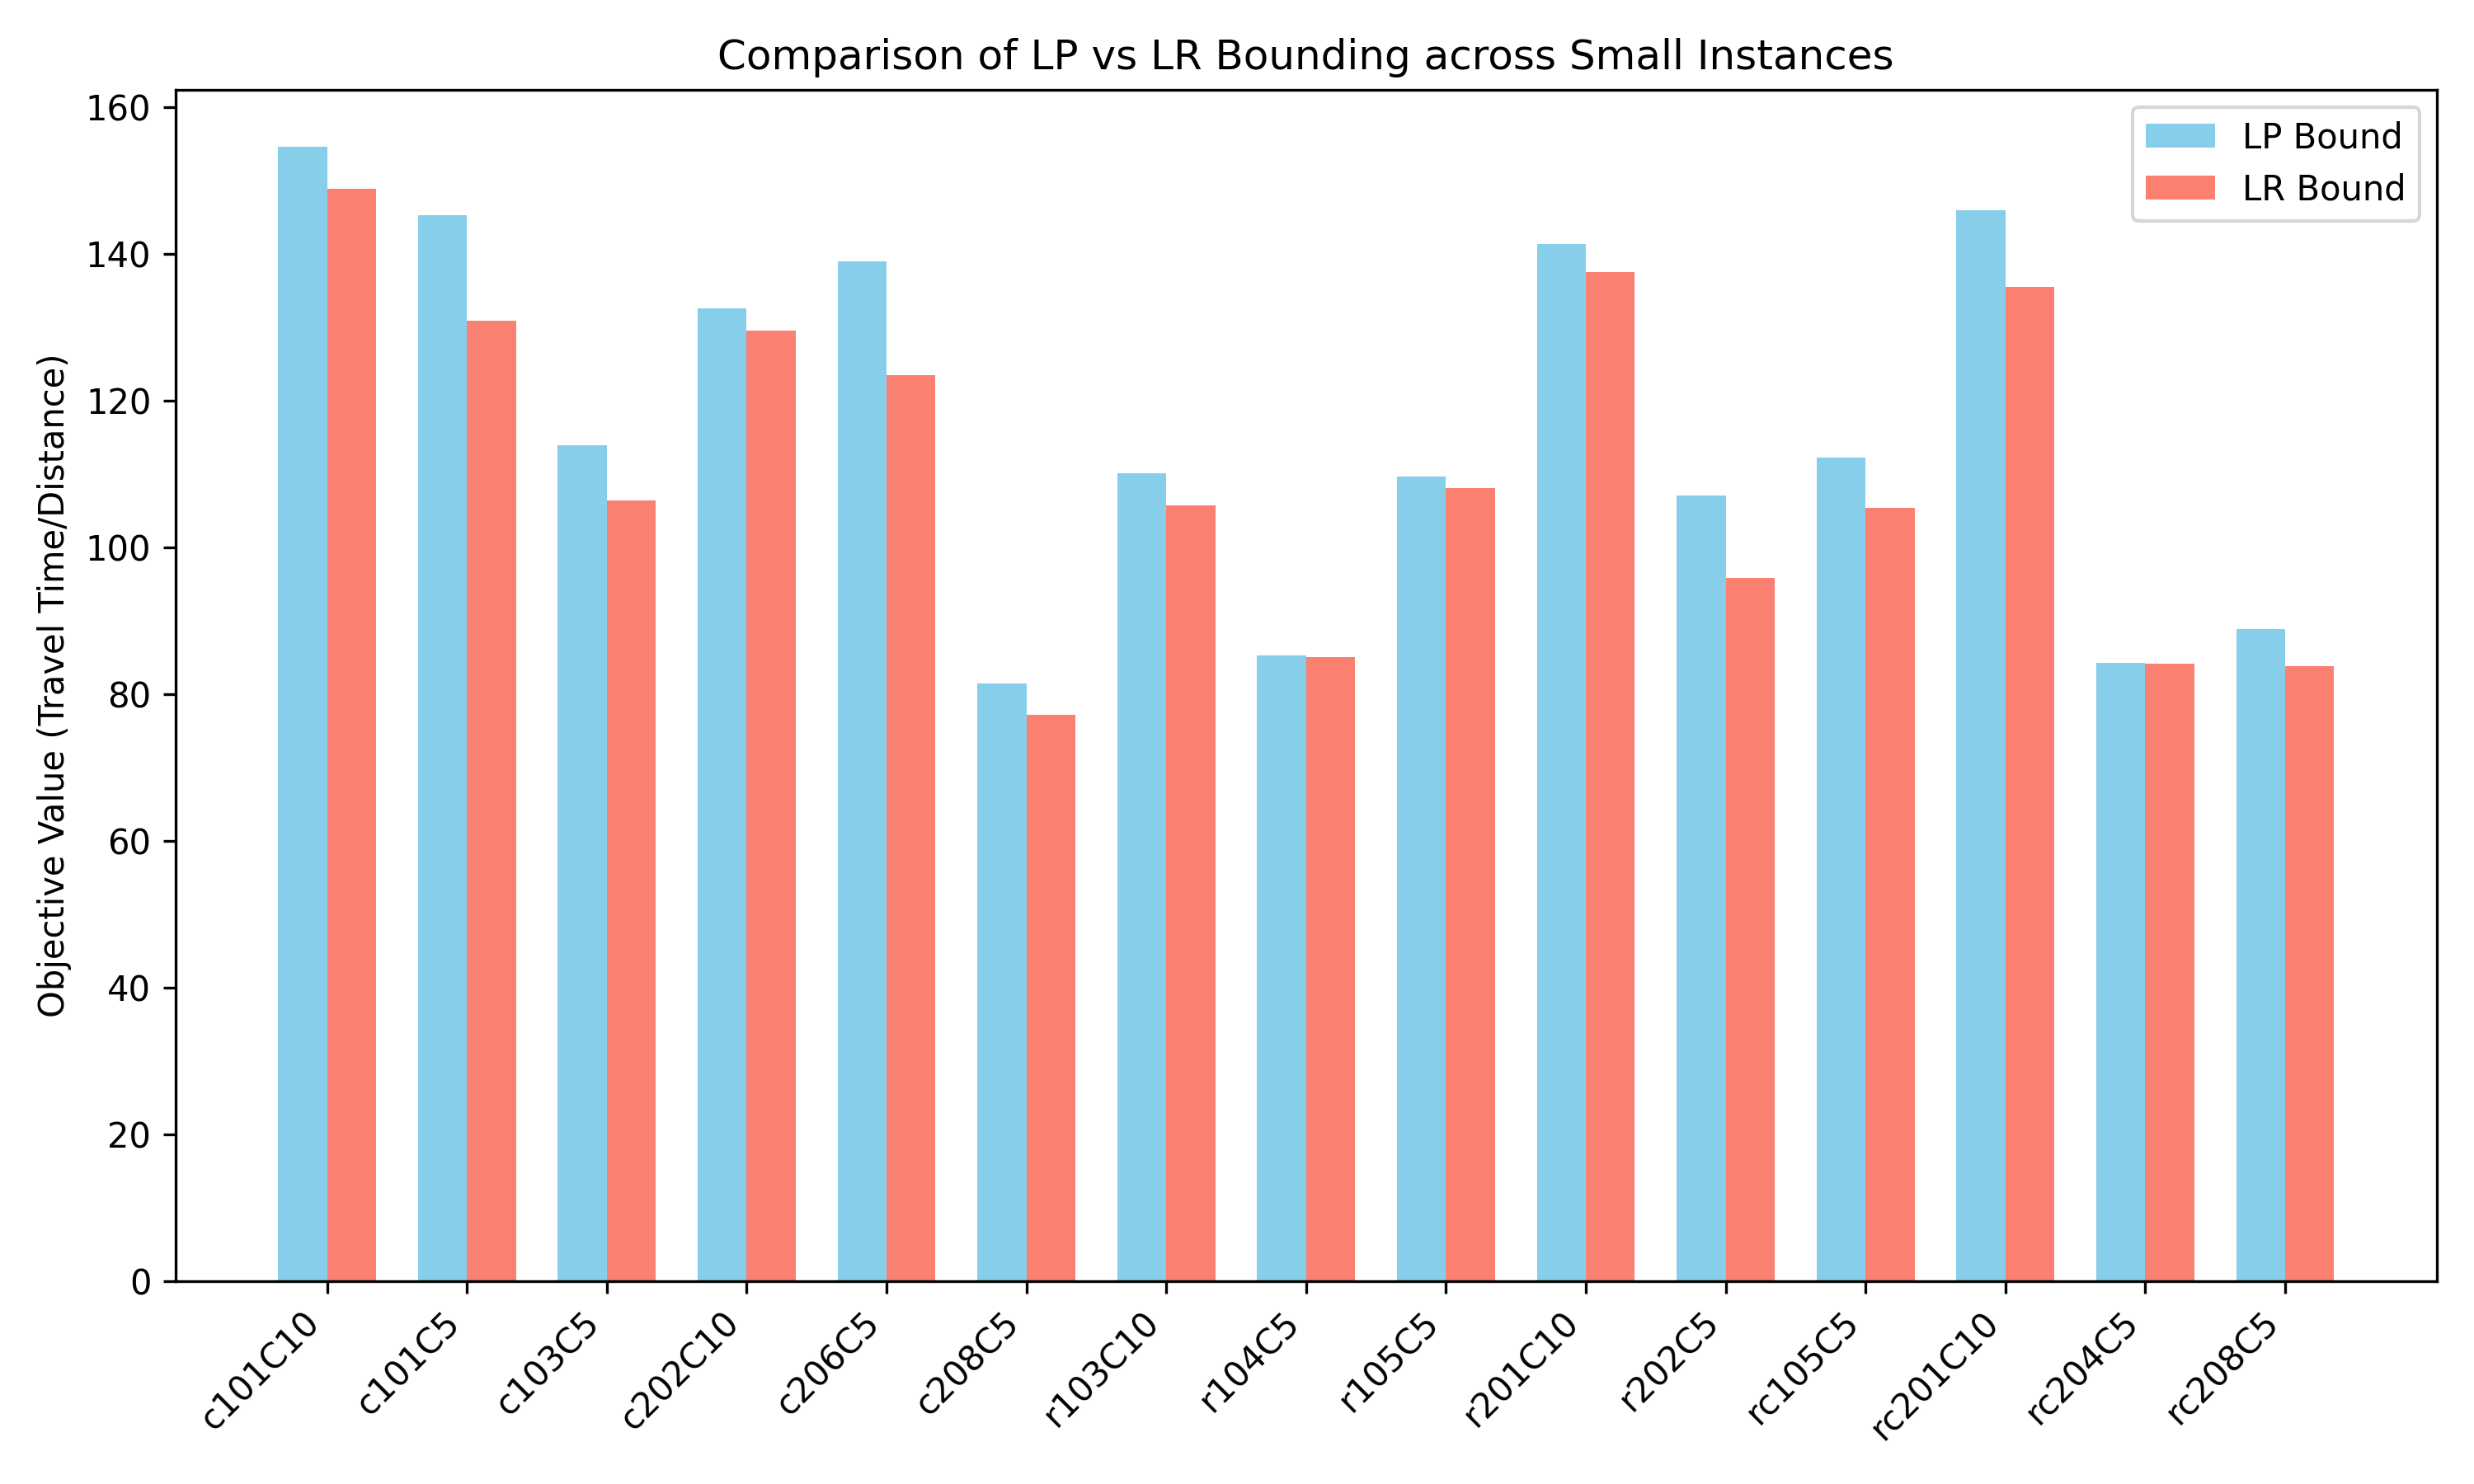
\includegraphics[width=0.8\textwidth]{duality_gap_plot.png}
    \caption{Empirical evaluation of the LP Bound vs our Lagrangian bounding execution convergence across all 15 valid instances.}
\end{figure}

\begin{table}[H]
    \centering
    \caption{Detailed Duality Gap Analysis across Valid Instances}
    \vspace{0.1cm}
    \begin{tabular}{@{}lccccc@{}}
    \toprule
    \textbf{Instance} & \textbf{Customers} & \textbf{LP Bound} & \textbf{LR Bound} & \textbf{Gap (\%)} & \textbf{LR Time (s)} \\
    \midrule
    \texttt{c101C10} & 10 & 154.68 & 148.88 & $-3.75\%$ & 2.89 \\
    \texttt{c101C5} & 5 & 145.36 & 130.93 & $-9.93\%$ & 2.13 \\
    \texttt{c103C5} & 5 & 113.93 & 106.46 & $-6.56\%$ & 2.09 \\
    \texttt{c202C10} & 10 & 132.68 & 129.64 & $-2.29\%$ & 2.84 \\
    \texttt{c206C5} & 5 & 139.03 & 123.52 & $-11.16\%$ & 2.24 \\
    \texttt{c208C5} & 5 & 81.48 & 77.23 & $-5.22\%$ & 2.21 \\
    \texttt{r103C10} & 10 & 110.20 & 105.77 & $-4.02\%$ & 2.86 \\
    \texttt{r104C5} & 5 & 85.28 & 85.09 & $-0.22\%$ & 2.39 \\
    \texttt{r105C5} & 5 & 109.70 & 108.11 & $-1.45\%$ & 2.32 \\
    \texttt{r201C10} & 10 & 141.44 & 137.54 & $-2.76\%$ & 3.00 \\
    \texttt{r202C5} & 5 & 107.10 & 95.84 & $-10.51\%$ & 2.39 \\
    \texttt{rc105C5} & 5 & 112.27 & 105.41 & $-6.11\%$ & 2.44 \\
    \texttt{rc201C10} & 10 & 146.01 & 135.57 & $-7.15\%$ & 2.91 \\
    \texttt{rc204C5} & 5 & 84.36 & 84.23 & $-0.15\%$ & 2.37 \\
    \texttt{rc208C5} & 5 & 88.94 & 83.84 & $-5.73\%$ & 2.33 \\
    \bottomrule
    \end{tabular}
\end{table}

\textbf{Solver Results}
\begin{itemize}
    \item The continuous LP relaxation provides a baseline bound by fully relaxing all geographic integer constraints. Across our 15 successful test cases, the Lagrangian bounds range from $-0.15\%$ to $-11.16\%$ from the optimal LP bound.
    \item The solver effectively drives up the Lagrangian lower bound starting from highly negative initialization values. Because our decomposed subproblem strips routing complexity directly down into flow conservation and set degree constraints, the subproblem inherits the \textbf{Integrality Property}. Consequently, optimization geometry dictates that the theoretical Lagrangian Dual bound exactly matches the continuous LP relaxation ($Z_{LR} = Z_{LP}$). Therefore, computationally, the iteratively optimized $Z_{LR}$ validly approaches $Z_{LP}$ asymptotically from below rather than surpassing it.
\end{itemize}

\subsection{Conclusion \& Future Works}
By exploiting the duality of the E-VRPTW, we offer computational convergence bounds for optimal geometries that standard route-optimization heuristics treat simply as black boxes. By extending this robust theoretical bounding groundwork via Dantzig-Wolfe decomposition and Branch-and-Price algorithms in future operations, the structural model can be vastly enhanced. Unlike standard subproblems, retaining the time windows recursively as an Elementary Shortest Path Problem with Resource Constraints (ESPPRC) effectively breaks the integrality property, granting access to strictly tighter optimal bounds crucial for orchestrating large-scale real-world EV logistics operations seamlessly.

\section*{References}
\begin{enumerate} [label={[\arabic*]}]
    \item Schneider, M., Stenger, A., \& Goeke, D. (2014). "The electric vehicle-routing problem with time windows and recharging stations." \textit{Transportation Science}, 48(4), 500-520.
    \item Verma, A. (2018). "Electric vehicle routing problem with time windows, recharging stations and battery swapping stations." \textit{EURO Journal on Transportation and Logistics}, 7(4), 415-451.
    \item Xiao, Y., Zhang, Y., Kaku, I., Kang, R., \& Pan, X. (2021). "Electric vehicle routing problem: A systematic review and a new comprehensive model with nonlinear energy recharging and consumption." \textit{Renewable and Sustainable Energy Reviews}, 151, 111567.
    \item Zhou, Y., Lei, Q., Li, L., \& Wu, Z. (2025). "An Overview of Energy Replenishment Strategies for the Electric Vehicle Routing Problem: Models and Solution Algorithms." \textit{Energies}, 18(23), 6196.
    \item Donval, V., Beraud, J.-F., Montenegro, T., \& Romet, P. (2026). "Ant Colony Optimization with Dynamic Pheromones for Electric Vehicle Routing and Charging Decisions." \textit{Sustainability}, 18(1), 417.
\end{enumerate}
\end{document}